\documentclass[a6paper, parskip=half, DIV=14, 10pt]{scrartcl}
\usepackage{fontspec}
\usepackage[dvipsnames]{xcolor}
\usepackage{tikz}

\usepackage{booktabs}
\usepackage{multicol}
\setlength\columnsep{3em}
\usepackage{enumitem}
\usepackage{caption}
\usepackage{scrlayer-scrpage} % Manage headers and footers in Koma-Script document classes
\setlength{\footskip}{1cm}

\usepackage[type={CC}, version={4.0}, modifier={by}]{doclicense} % Add text and icons for creative commons license
\usepackage{array}
\usepackage{afterpage}

\usepackage{pg32}
\usepackage{contour}
\contournumber{32}
\usepackage[letterspace=50]{microtype}

\usepackage[hidelinks]{hyperref} % Add hyperlinks to the pdf file. This should usually be the last package loaded before \begin{document}

\setmainfont{TeX Gyre Schola}
\makeatletter
\newcommand{\version}[1]{\newcommand{\@version}{#1}}
\makeatother

% Set header
\clearpairofpagestyles
\makeatletter
\cfoot*{\normalshape Version \@version}
\makeatother

% Minimize unwanted hyphenation
\tolerance=1
\emergencystretch=\maxdimen
\hyphenpenalty=10000
\hbadness=10000

\setkomafont{section}{\setmainfont{Tex Gyre Schola}\Large\bfseries}
\setkomafont{subsection}{\setmainfont{Tex Gyre Schola}\large\bfseries}
\setkomafont{subsubsection}{\setmainfont{Tex Gyre Schola}\normalsize\bfseries}
\setkomafont{descriptionlabel}{\setmainfont{Tex Gyre Schola}\normalsize\bfseries}

\RedeclareSectionCommand[
  runin=false,
  afterindent=false,
  beforeskip=0cm,
  afterskip=0ex,
]{section}

\RedeclareSectionCommand[
  runin=false,
  afterindent=false,
  beforeskip=0pt,
  afterskip=0ex,
]{subsection}

\RedeclareSectionCommand[
  runin=false,
  afterindent=false,
  beforeskip=0pt,
  afterskip=0ex,
]{subsubsection}

\version{0.1}
\begin{document}
\color{offblack}
{%
\thispagestyle{empty}
		\enlargethispage{3.5\baselineskip} % Move the bottom line (author and date) down a bit
\setmainfont[Scale=1.0]{Tex Gyre Schola}
\begin{center}
\makeatletter
{Version \@version}
\makeatother

\vspace{0.5cm}

\setmainfont[Scale=2.9]{Tex Gyre Schola}
\Huge
\contour{offblack}{\textcolor{offblue}{\textls{Pivot}}}\hspace{1.65cm}

\vspace{0.2cm}

\contour{offblack}{\textcolor{offgreen}{\textls{Pawns}}}
\vfill{}

\scalebox{-1}[1]{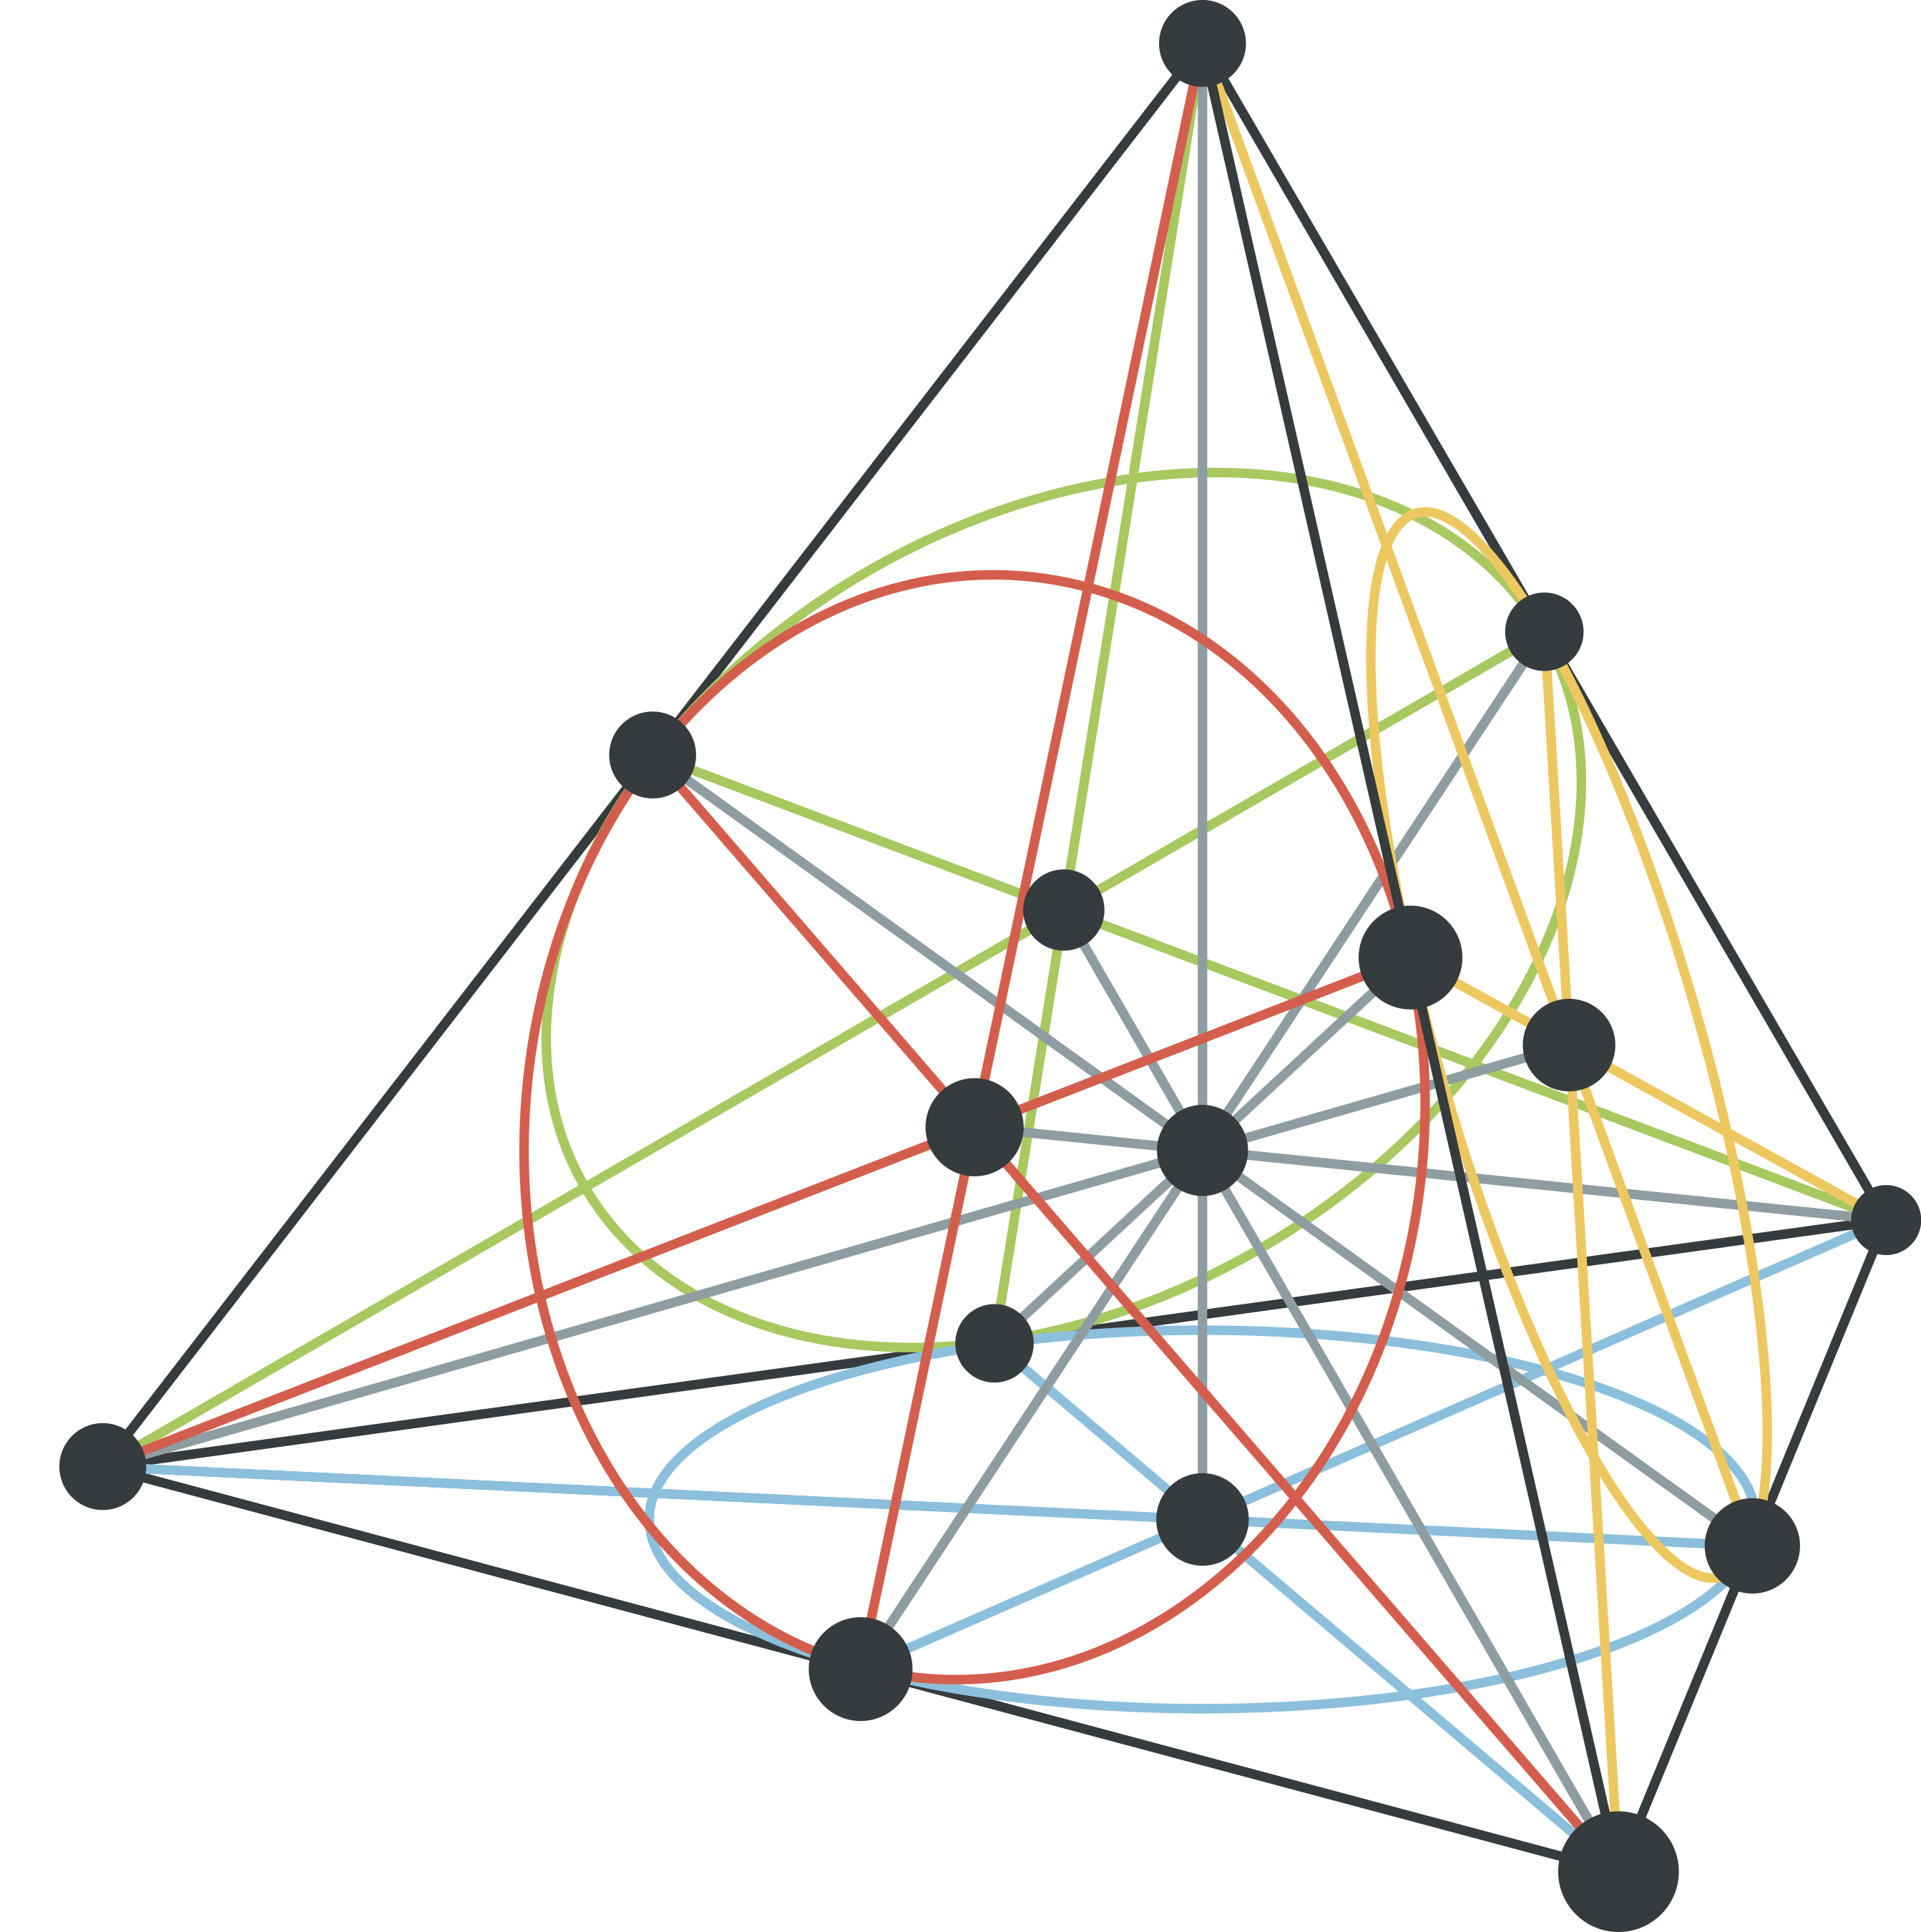
\includegraphics[scale=0.0625]{Images/pg32_tetrahedron.png}}
\vfill{}
\tiny
Designed by Michael Purcell\hspace*{1.5cm}
\end{center}
}%
%\newpage
%\thispagestyle{empty}
%\phantom{a}

\newpage
\setmainfont{Tex Gyre Schola}%
\raggedright%
\section*{Components}
\begin{itemize}[leftmargin=*, noitemsep]
	\item 15 cards
      \begin{itemize}[leftmargin=*]
        \item Each card displays seven different icons, a \emph{centre icon} and six other icons.% which are arranged in a hexagon around the centre icon.
        \item Each icon is displayed on three different cards.
        \item For every pair of cards, there is exactly one icon that is displayed on both cards.
        \item There are a total of thirty-five different icons.
        \item Each icon is rendered in one of five colours: red, green, blue, yellow, or black.
      \end{itemize}
    \item 15 target tokens
    \begin{itemize}[leftmargin=*]
      \item Each target token displays one icon.
    \end{itemize}
  \item 5 pawns
      \begin{itemize}[leftmargin=*]
        \item There is one pawn in each of the icon colours.
      \end{itemize}
  \item 5 placeholder tokens
      \begin{itemize}[leftmargin=*]
        \item There is one placeholder token in each of the icon colours.
      \end{itemize}
  \item 1 sand timer (approximately thirty seconds)
  \item 1 cloth bag
\end{itemize}

\newpage

\section*{Overview}
Pivot Pawns is a find-the-match puzzle game for any number of players. Pivot Pawns can be played in 15-30 minutes and is intended for players who are at least eight years old.

\section*{Set Up}
\begin{enumerate}[leftmargin=*]
	\item Shuffle the cards.
	\item Deal the cards face up on the table in a tableau consisting of three rows and five columns.
	\item Put the sand timer beside the tableau.
	\item Put the target tokens into the cloth bag.
	\item Place each pawn on one of the starting cards.
	\begin{itemize}[leftmargin=*]
	  \item The centre icons of the starting cards are the following: music notes, flask, Mars symbol, leaf, and sun.
	  \item Place each pawn on a card which has a centre icon of a different colour to that pawn.
	  \item Do not place more than one pawn on any card.
	\end{itemize}
	\item Place each placeholder token on the card where you placed the pawn of the same colour.
\end{enumerate}

\newpage

\section*{Playing the Game}
The game takes place over of fifteen \emph{rounds}.

During each round, your objective is to collect the target token for that round. To do so, you must move the \emph{active pawn} onto the \emph{target card}. The active pawn is the pawn that matches the colour of the icon displayed on the target token. The target card is the card that displays the icon on the target token in its centre.

The game ends after you have played fifteen rounds. Whoever has collected the most target tokens at the end of the game wins.

\subsection*{Moving the Pawns}
During the game, you will move the pawns around the tableau. When a pawn is placed onto a card, that card is \emph{occupied} by that pawn.

Unless it is the target card for a given round, you may not move a pawn onto a card which has a centre icon of the same colour as that pawn.

Crucially, however, you may move any pawn onto the target card during a given round. In fact, in order to collect the target token in each round, you must move the pawn that matches the colour of the centre icon of the target card onto that card.

\newpage

To move a pawn, you perform an action called a \emph{pivot} by doing the following:
\begin{enumerate}[leftmargin=*]
  \item Identify the \emph{moving pawn}. The moving pawn is the pawn that you will move with this pivot.
  \item Identify the \emph{pivot pawn}. The pivot pawn determines how you can move the moving pawn.
  \item Identify the \emph{pivot icon}. The pivot icon is the icon that is displayed on the cards occupied by the moving pawn and the pivot pawn.
  \item Identify the \emph{destination card}. The destination card is the card that displays the pivot icon and is not occupied by either the moving pawn or the pivot pawn.
  \item Place the moving pawn on the destination card.
\end{enumerate}

\textbf{Notes:}
\begin{enumerate}[leftmargin=*]
  \item Each card may be occupied by at most one pawn.
  \item You may not move the moving pawn onto a card that is occupied by another pawn.
\end{enumerate}

\newpage

\subsection*{Playing a Round}
At the beginning of each round, first draw a target token from the cloth bag and place it on the table. The round is then divided into three \emph{phases}.

\subsubsection*{Phase 1}
During the first phase, the pawns move only in your minds. You should study the tableau and try to find a \emph{solution}. A solution is a series of pivots that delivers the active pawn to the target card.

\textbf{Notes:}
\begin{itemize}[leftmargin=*]
  \item A solution may involve moving any of the pawns.
%  \item The shortest solution will usually involve moving at least one pawn that is not the active pawn for that round.
\end{itemize}

\subsubsection*{Phase 2}
The second phase begins when someone finds a solution.
That player should place a \emph{bid} by stating the number of pivots for their solution and then turn the sand timer over.
Everyone will then have thirty seconds to make additional bids.

\textbf{Notes:}
  \begin{itemize}[leftmargin=*]
    \item There is no order of bidding.
    \item You may make multiple bids.
    \item Once you have made a bid for a given round, you may not change it to a higher number.   
  \end{itemize}

\newpage

\subsubsection*{Phase 3}
The third phase begins when the sand timer runs out. The player with the lowest bid should attempt to \emph{demonstrate} their solution (see below).

If their proposed solution is valid, then that player \emph{succeeds} and should collect the target token for the round. Otherwise, the player with the next lowest bid should attempt to demonstrate their solution. This continues until someone succeeds.

\textbf{Notes:}
  \begin{itemize}[leftmargin=*]
  \item If no one succeeds, then no one gets the target token for that round.
  \item If two or more players have the same bid, then the bids should be resolved in the order in which they were were made.
  \end{itemize}

\vfill
\hrulefill
\subsection*{About the Cover}
The design of the cards used in Pivot Pawns is derived from the geometry of the three-dimensional projective space over the finite field with two elements. This space is known as PG(3,2). 

One way to understand PG(3,2) is as a tetrahedron like the one depicted on the cover of this rulebook. 

\newpage

\subsection*{Demonstrating a Solution}
To demonstrate a solution, you should execute the pivots required to move the active pawn onto the target card, counting aloud as you make each move. You should identify the moving pawn, the pivot pawn, and pivot icon for each move.

Your solution is \emph{valid} if all moves are legal and the solution delivers the active pawn to the target card in less than or equal to the number of moves you have bid. Otherwise it is \emph{invalid}.

If, while demonstrating your solution, you make a mistake or discover that your solution is invalid, you should return the pawns to their original locations as indicated by the placeholder tokens.

If your solution is valid, then you should update the locations of the placeholder tokens by placing them on the same cards as their corresponding pawns.


\vfill
\hrulefill

\textbf{Game Design}: Michael Purcell\\
\textbf{Contact}: \href{mailto:pivot.pawns@gmail.com}{pivot.pawns@gmail.com}\\
\begin{tabular}{@{}m{\columnwidth-\widthof{\Huge{\doclicenseIcon}}-0.5cm}@{\hspace{0.05cm}}m{\widthof{\Huge{\doclicenseIcon}}}@{}}
{\textbf{License}: This work is licensed\newline under a ``CC BY 4.0'' license.} & \Huge{\doclicenseIcon}\\
\end{tabular}

%\newpage
%\thispagestyle{empty}
%\phantom{a}
%
%\newpage
%\thispagestyle{empty}
%\phantom{a}
\end{document}
